% 75-26(75쪽) — $0\le x\le 2\pi$ 에서 $y=\sin x$, $y=\cos x$ 와 직선 $y=k$(원문 「오른쪽 그림」). 스캔 화질이 낮아 TikZ 로 다시 그림.
% 라벨은 원문 것만: $1$, $-1$, $\pt{O}$, $a$, $b$, $c$, $d$, $2\pi$, 세 그래프 이름. 가로축 단위는 $\pi$ 배.
% $a$, $b$, $c$, $d$ 의 값은 원문처럼 적지 않는다(답이 그림에서 읽히지 않게).
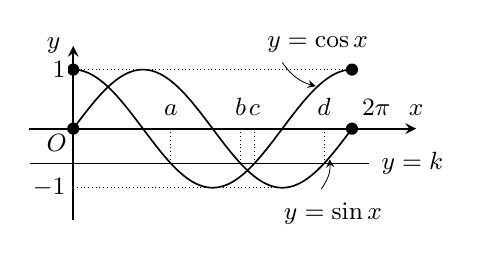
\begin{tikzpicture}[line width=0.6pt, x=1.77cm, y=0.75cm, >=stealth]
  \draw[densely dotted, line width=0.35pt] (0,1) -- (2,1);
  \draw[densely dotted, line width=0.35pt] (0,-1) -- (1.5,-1);
  \draw[->, line width=0.7pt] (-0.32,0) -- (2.46,0) node[above=1pt, font=\small] {$x$};
  \draw[->, line width=0.7pt] (0,-1.55) -- (0,1.40) node[left=1pt, font=\small] {$y$};
  \draw[line width=0.5pt] (-0.31,-0.5878) -- (2.12,-0.5878);
  \draw[domain=0:2, samples=200, smooth] plot (\x, {sin(180*\x)});
  \draw[domain=0:2, samples=200, smooth] plot (\x, {cos(180*\x)});
  \foreach \t in {0.7,1.2,1.3,1.8}{
    \draw[densely dotted, line width=0.35pt] (\t,0) -- (\t,-0.5878);
  }
  \fill (0,1) circle (2.2pt);
  \fill (0,0) circle (2.2pt);
  \fill (2,1) circle (2.2pt);
  \fill (2,0) circle (2.2pt);
  \node[anchor=east, font=\small, fill=white, inner sep=1pt] at (-0.03,1) {$1$};
  \node[anchor=east, font=\small, fill=white, inner sep=1pt] at (-0.03,-1) {$-1$};
  \node[anchor=north east, font=\small, fill=white, inner sep=0.5pt] at (-0.03,-0.06) {$\pt{O}$};
  \node[anchor=south, font=\small] at (0.70,0.05) {$a$};
  \node[anchor=south, font=\small] at (1.20,0.05) {$b$};
  \node[anchor=south, font=\small] at (1.30,0.05) {$c$};
  \node[anchor=south, font=\small] at (1.80,0.05) {$d$};
  \node[anchor=south west, font=\small] at (2.00,0.05) {$2\pi$};
  \node[anchor=west, font=\small] at (2.14,-0.5878) {$y=k$};
  \node[anchor=south west, font=\small] at (1.32,1.12) {$y=\cos x$};
  \draw[->, line width=0.3pt] (1.50,1.12) to[bend right=20] (1.74,0.72);
  \node[anchor=north west, font=\small] at (1.44,-1.08) {$y=\sin x$};
  \draw[->, line width=0.3pt] (1.78,-1.02) to[bend right=20] (1.84,-0.52);
\end{tikzpicture}
